\documentclass{standalone}

\usepackage{xcolor}

\definecolor{myblue}{HTML}{377EB8}
\definecolor{myred}{HTML}{E41A1C}
\definecolor{myviolet}{HTML}{984EA3}
\definecolor{myteal}{HTML}{008B8B}

\usepackage{tikz}
\usepackage{pgfplots}
\pgfplotsset{compat=newest}

\usepackage{lmodern}
\SetSymbolFont{letters}{bold}{OML}{cmbr}{bx}{it}
\renewcommand{\familydefault}{\sfdefault}

\usepackage{sansmathfonts}

\begin{document}
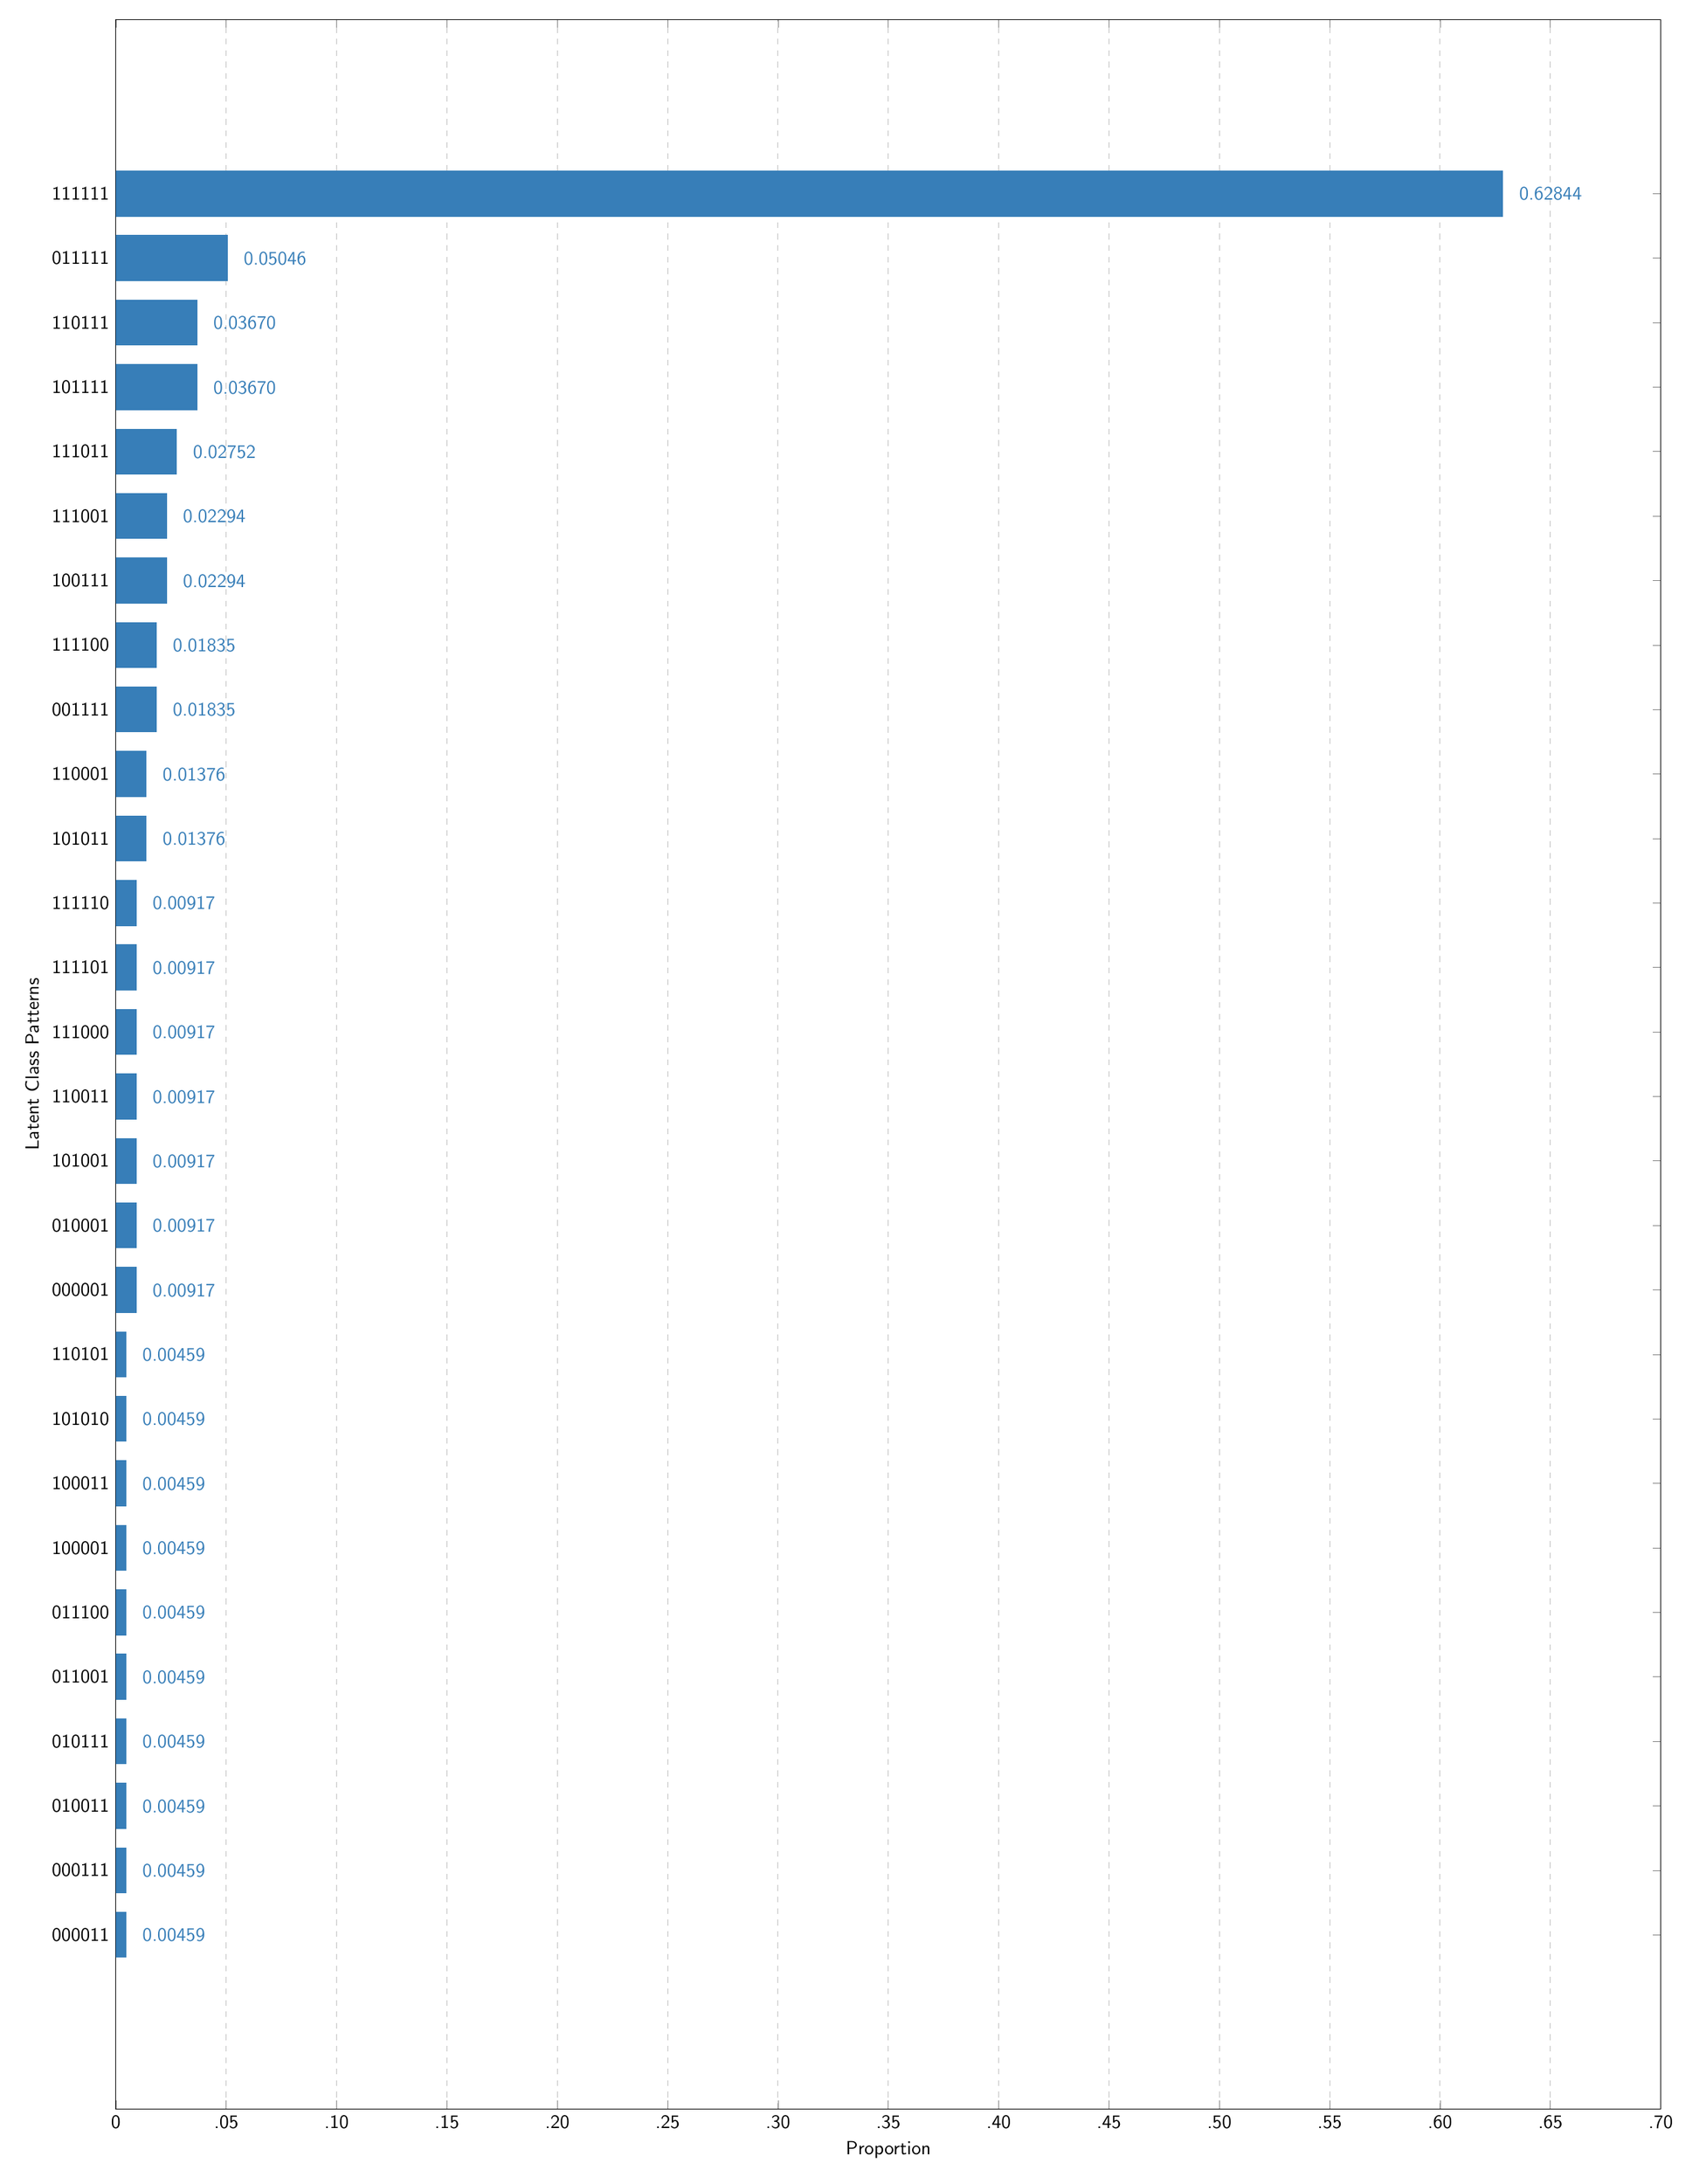
\begin{tikzpicture}
	\begin{axis}[
			xlabel={Proportion},
			ylabel={Latent Class Patterns},
			xmin=0,
			xmax=0.7,
			xtick={
				0,
				.05,
				.10,
				.15,
				.20,
				.25,
				.30,
				.35,
				.40,
				.45,
				.50,
				.55,
				.60,
				.65,
				.70
			},
			xticklabels={
				0,
				.05,
				.10,
				.15,
				.20,
				.25,
				.30,
				.35,
				.40,
				.45,
				.50,
				.55,
				.60,
				.65,
				.70
			},
			ytick={
				1,
				2,
				3,
				4,
				5,
				6,
				7,
				8,
				9,
				10,
				11,
				12,
				13,
				14,
				15,
				16,
				17,
				18,
				19,
				20,
				21,
				22,
				23,
				24,
				25,
				26,
				27,
				28
			},
			yticklabels={
				000011,
				000111,
				010011,
				010111,
				011001,
				011100,
				100001,
				100011,
				101010,
				110101,
				000001,
				010001,
				101001,
				110011,
				111000,
				111101,
				111110,
				101011,
				110001,
				001111,
				111100,
				100111,
				111001,
				111011,
				101111,
				110111,
				011111,
				111111
			},
			width=30cm,
			height=40cm,
			bar width=0.7,
			ymajorgrids=false,
			xmajorgrids=true,
			grid style=dashed,
			nodes near coords,
			nodes near coords align={horizontal},
			every node near coord/.append style={xshift=25pt, yshift=-7pt},
			point meta=explicit symbolic,
		]
		\addplot[myblue, xbar, fill=myblue] coordinates {
			(0.00459,1)[0.00459]
			(0.00459,2)[0.00459]
			(0.00459,3)[0.00459]
			(0.00459,4)[0.00459]
			(0.00459,5)[0.00459]
			(0.00459,6)[0.00459]
			(0.00459,7)[0.00459]
			(0.00459,8)[0.00459]
			(0.00459,9)[0.00459]
			(0.00459,10)[0.00459]
			(0.00917,11)[0.00917]
			(0.00917,12)[0.00917]
			(0.00917,13)[0.00917]
			(0.00917,14)[0.00917]
			(0.00917,15)[0.00917]
			(0.00917,16)[0.00917]
			(0.00917,17)[0.00917]
			(0.01376,18)[0.01376]
			(0.01376,19)[0.01376]
			(0.01835,20)[0.01835]
			(0.01835,21)[0.01835]
			(0.02294,22)[0.02294]
			(0.02294,23)[0.02294]
			(0.02752,24)[0.02752]
			(0.03670,25)[0.03670]
			(0.03670,26)[0.03670]
			(0.05046,27)[0.05046]
			(0.62844,28)[0.62844]
		};
	\end{axis}
\end{tikzpicture}
\end{document}
